\documentclass{amsart}
\usepackage[utf8]{inputenc}
\usepackage{enumitem}
\usepackage{physics}
\usepackage{bm}
\usepackage{bbm}
\usepackage{hyperref}
\usepackage{tikz} 
\usetikzlibrary{positioning, arrows, matrix, intersections}
\usepackage{tabularx}
\newcolumntype{C}{>{\centering\arraybackslash}X}
\usepackage{xfrac}
\usepackage{adjustbox}
\usepackage{mathpartir}
\usepackage{quiver}
\usepackage{multicol}
\usepackage{amsmath}
\usepackage{pifont}
\newcommand{\cmark}{\ding{51}}%
\newcommand{\xmark}{\ding{55}}

\tikzset{snake it/.style={decorate, decoration=snake}}

\usepackage{minted}
\usemintedstyle{tango}

\theoremstyle{definition}
\newtheorem{eg}{Example}[section]
\newtheorem{ex}{Exercise}[section]
\newtheorem{defn}{Definition}[section]
\newtheorem*{sol}{Solution}
\newtheorem*{warn}{Warning}
\newtheorem*{fact}{Fact}
\newtheorem*{cor}{Corollary}

\usepackage{pgfplots}
\pgfplotsset{compat=1.12}
\usepgfplotslibrary{fillbetween}

\title[Introduction to HoTT Notes]{OPLSS 2023 \\
Introduction to HoTT Notes}
\author{Pavel Kovalev, Sean O'Connor, Cassia Torczon, Frank Tsai}
\date{July 2023}


\newcommand{\N}{\mathbbm{N}}
\newcommand{\Z}{\mathbbm{Z}}
\newcommand{\Q}{\mathbbm{Q}}
\newcommand{\R}{\mathbbm{R}}
\newcommand{\ctx}{\ensuremath{\mathsf{~ctx}}}
\newcommand{\type}{\ensuremath{\mathsf{~type}}}
\newcommand{\defeq}{\ensuremath{\overset{\boldsymbol{\cdot}}{=}}}
\newcommand{\Unit}{\ensuremath{\mathbbm{1}}}
\newcommand{\Bool}{\ensuremath{\mathsf{Bool}}}
\newcommand{\Prop}{\ensuremath{\mathsf{Prop}}}
\newcommand{\isProp}{\ensuremath{\mathsf{isProp}}}
\newcommand{\Set}{\ensuremath{\mathsf{Set}}}
\newcommand{\isSet}{\ensuremath{\mathsf{isSet}}}
\newcommand{\Cat}{\ensuremath{\mathsf{Cat}}}
\newcommand{\isContr}{\ensuremath{\mathsf{isContr}}}
\newcommand{\isGroupoid}{\ensuremath{\mathsf{isGroupoid}}}
\newcommand{\Rezk}{\ensuremath{\mathsf{Rezk}}}
\newcommand{\isofhlevel}[2]{\ensuremath{\mathsf{isofhlevel}~#1~#2}}
\newcommand{\isEquiv}{\ensuremath{\mathsf{isEquiv}}}
\newcommand{\idToEquiv}{\ensuremath{\mathsf{idToEquiv}}}
\newcommand{\idToIso}{\ensuremath{\mathsf{idToIso}}}
\newcommand{\Iso}{\ensuremath{\mathsf{Iso}}}
\newcommand{\Grp}{\ensuremath{\mathsf{Grp}}}
\newcommand{\Grpd}{\ensuremath{\mathsf{Grpd}}}
\newcommand{\W}{\ensuremath{\mathsf{W}}}
\newcommand{\U}{\ensuremath{\mathcal{U}}}
\newcommand{\True}{\ensuremath{\mathsf{true}}}
\newcommand{\False}{\ensuremath{\mathsf{false}}}
\newcommand{\Ind}{\ensuremath{\mathsf{ind}}}
\newcommand{\Hole}[1]{\fbox{?#1}}
\newcommand{\ob}[1]{\ensuremath{\mathrm{ob}{(\cat{#1})}}}
\newcommand{\cHom}[2]{\ensuremath{\mathrm{hom}(#1,#2)}}
\newcommand{\cId}{\ensuremath{\mathbf{1}}}
\newcommand{\ua}{\ensuremath{\mathsf{ua}}}
\newcommand{\cat}[1]{\ensuremath{\mathbf{#1}}}
\newcommand{\inl}{\ensuremath{\mathsf{inl}}}
\newcommand{\inr}{\ensuremath{\mathsf{inr}}}
\renewcommand{\emph}{\textbf}
\renewcommand{\emptyset}{\varnothing}

\newcommand{\newcommenter}[3]{%
  \newcommand{#1}[1]{%
    \textcolor{#2}{\small\textsf{[{#3}: {##1}]}}%
  }%
}
\newcommenter{\FT}{red}{FT}

\usepackage[normalem]{ulem}
\newcommand{\surprising}{\textcolor{blue}{s\uwave{urprisin}g} $\text{}$}

\begin{document}

\maketitle
\tableofcontents

\section{Introduction}
\label{sec:introduction}

The fields of Type theory, Set theory, Topos theory, Category theory, Homotopy theory, and Functional programming all matured in the 20th century as their own distinct and influential fields of study. But near the beginning of the 21st century, more and more of the connections across these fields were recognized, which years later culminated in the field of Homotopy Type Theory (HoTT).

\begin{figure}[h]
    \centering
    \[\begin{tikzcd}
	{\text{Type theory}} & {\text{Logic}} & {\text{Set theory}} \\
	{\text{Functional programming}} & {\text{HoTT}} & {\text{Topos theory}} \\
	{\text{Homotopy theory}} && {\text{Category theory}}
	\arrow[no head, from=3-1, to=2-2]
	\arrow[no head, from=2-1, to=2-2]
	\arrow[no head, from=1-1, to=2-2]
	\arrow[no head, from=1-2, to=2-2]
	\arrow[no head, from=1-3, to=2-2]
	\arrow[no head, from=2-3, to=2-2]
	\arrow[no head, from=3-3, to=2-2]
	\arrow[no head, from=1-1, to=1-2]
	\arrow[no head, from=1-2, to=1-3]
	\arrow[no head, from=1-3, to=2-3]
	\arrow[no head, from=2-3, to=3-3]
	\arrow[no head, from=3-3, to=3-1]
	\arrow[no head, from=1-1, to=2-1]
	\arrow[color={rgb,255:red,0;green,0;blue,255}, shorten <=0pt, squiggly, no head, from=3-1, to=2-1]
\end{tikzcd}\]
    \caption{Connections across different fields of mathematics and computer science.
    The blue squiggly line is the surprising connection between homotopy theory and functional programming.}
    \label{fig:connections-across-fields}
\end{figure}

HoTT has strong ties to each of these other fields, and provides a fertile ground for investigating and proving \surprising connections between each of them. This lecture series will provide an introduction to this growing field and will help illuminate its relation to these other areas of study.
HoTT is built on top of Martin-L\"{o}f Type Theory (MLTT), which we introduce in \S\ref{sec:martin-lof-type-theory}.


\section{Martin-L\"{o}f Type Theory}
\label{sec:martin-lof-type-theory}
MLTT consists of 3 basic judgments.
An in-depth treatment of judgments can be found in \cite{ml:justif-log}.
The first judgment expresses that $\Gamma$ is a valid context.
\[
\Gamma \ctx
\]
The second judgment expresses that $T$ is a type under the context $\Gamma$, presupposing that $\Gamma \ctx$.
\[
\Gamma \vdash T \type
\]
Finally, the last judgment expresses that $t$ is an element of type $T$ under the context $\Gamma$, presupposing that $\Gamma \ctx$ and that $\Gamma \vdash T \type$.
\[
\Gamma \vdash t : T
\]
These three judgments have their corresponding equality judgments.
The first judgment expresses that two valid contexts, $\Gamma$ and $\Gamma'$, are definitionally equal.
\[
\Gamma \defeq \Gamma' \ctx
\]
The second judgment expresses that two types are definitionally equal under the same context $\Gamma$.
\[
\Gamma \vdash T \defeq T' \type
\]
And the last judgment expresses that two terms, $t$ and $t'$, of type $T$ under the context $\Gamma$ are definitionally equal.
\[
\Gamma \vdash t \defeq t' : T
\]
For conciseness, we omit the context $\Gamma$.
For example, we write $\vdash t : T$ for $\Gamma \vdash t : T$, where $\Gamma$ is an arbitrary context.
\begin{eg}[Some example types in MLTT]
\hfill
\begin{multicols}{2}
\begin{enumerate}
\item Empty type $\varnothing$.
\item Unit type $\Unit$.
\item The type of Boolean $\Bool$.
\item The type of natural numbers $\N$.
\item The types of equalities $=$.
\item Dependent product types $\Sigma$.
\item Dependent function types $\Pi$.
\item Universes $\U_{i}$.
\end{enumerate}
\end{multicols}
\vspace{-\baselineskip}
\begin{enumerate}
    \item[(5)] The types of well-founded trees $\W$. 
\end{enumerate}
\end{eg}

MLTT can be extended with additional features.
Two possible extensions are summarized in Table \ref{tb:extensions-of-mltt}.
\begin{table}[h]
    \centering
    \begin{tabular}{|c||c|c|}\hline
        Type Theory & Univalence Axiom & Higher Inductive Types\\\hline
        UTT  & \cmark & \xmark\\\hline
        HoTT & \cmark & \cmark\\\hline
    \end{tabular}
    \caption{Univalent Type Theory (UTT) is MLTT extended with the Univalence Axiom, and HoTT is UTT extended with higher inductive types.}
    \label{tb:extensions-of-mltt}
\end{table}

\subsection{Inductive Types}
\label{sec:inductive-types}
An inductive type is freely generated by its canonical elements.
To define an inductive type in Coq, one can write
\begin{figure}[H]
    \centering
    \begin{minted}{coq}
        Inductive T : Type := foo : T | bar : T.
    \end{minted}
\end{figure}
The type \texttt{T} is freely generated by its two canonical elements, namely \texttt{foo} and \texttt{bar}.
Coq generates an elimination rule for \texttt{T} automatically.

In general, to specify a new type in type theory we specify:
\begin{enumerate}
    \item how to form new types of this kind via \emph{formation rules}.
    For example, if $A$ and $B$ are types then $A \to B$ is a type.
    \item how to construct canonical elements of that type via \emph{introduction rules}.
    For example, a function type has one introduction rule, namely $\lambda$-abstraction.
    \item how to use elements of that type via \emph{elimination rules}.
    For example, a function type has one elimination rule, namely function application.
    \item how elimination rules act on introduction rules via \emph{computation rules}.
    For example, applying a $\lambda$-abstraction $(\lambda x.e)$ to a term $e'$ is definitionally equal to substituting $e'$ for $x$ in $e$, namely $e[\sfrac{e'}{x}]$. 
\end{enumerate}
See the HoTT book \cite{hottbook}.

\subsection{The Booleans}
\label{sec:the-booleans}

The type $\Bool$ is freely generated by two terms, $\True$ and $\False$.
To use a Boolean (to construct a dependent function out of $\Bool$), it suffices to specify its behaviors on the canonical terms.
The computation rules express that $\Ind_{\Bool,f,t}(b)$ works as expected when applied to one of the canonical terms.

\begin{mathpar}
    \inferrule*[Right=Form]{ }{\vdash \Bool \type} \and

    \inferrule*[Right=Intros]{ }
    { \vdash \True : \Bool \and 
      \vdash \False : \Bool
    }\and

    \inferrule*[Right=Elim]
    { b : \Bool \vdash D(b) \type \\
      \vdash f : D(\False) \\
      \vdash t : D(\True)
    }
    { b : \Bool \vdash \Ind_{\Bool,f,t}(b) : D(b) } \and

    \inferrule*[Right=Comp]
    { b: \Bool \vdash D(b) \type \\
      \vdash f : D(\False) \\ 
      \vdash t : D(\True)
    }
    { \vdash \Ind_{\Bool,f,t}(\False) \defeq f : D(\False) \and
      \vdash \Ind_{\Bool,f,t}(\True) \defeq t : D(\True) }
\end{mathpar}

\begin{ex}\label{ex:not}
    Define a function $\mathsf{not}: \Bool \to \Bool$.
    Note that $\to$ works as usual.
\end{ex}

\subsection{The Natural Numbers}
\label{sec:the-natural-numbers}

The type $\N$ is freely generated by $0$ and the successor function $S$.
One may recognize that the elimination rule is the usual mathematical induction.
\begin{mathpar}
    \inferrule*[Right=Form]{ }
    { \vdash \N \type }\and

    \inferrule*[Right=Intros]{ }
    { \vdash 0 : \N }\and

    \inferrule*[Right=Intros]
    { \vdash n : \N }
    { \vdash S(n) : \N }\and

    \inferrule*[Right=Elim]
    { n : \N \vdash D(n) \type \\
      \vdash z : D(0) \\
      n : \N, h : D(n) \vdash i : D(S(n))
    }
    { n : \N \vdash \Ind_{\N,z,i}(n) : D(n) }\and

    \inferrule*[Right=Comp]
    { n : \N \vdash D(n) \type \\
      \vdash z : D(0) \\
      n : \N, h : D(n) \vdash i : D(S(n))
    }
    { \Ind_{\N,z,i}(0) \defeq z : D(0) \and
      n : \N \vdash \Ind_{\N,z,i}(S(n)) \defeq i[\sfrac{\Ind_{\N,z,i}(n)}{h}] : D(S(n)) }
\end{mathpar}

\begin{eg}\label{eg:add}
    To construct a function $\mathsf{add} : \N \to \N \to \N$, it suffices to construct a term $n : \N, m : \N \vdash e : \N$.
    To this end, we do induction on $m$ (apply the elimination rule for $\N$), choosing $n : \N, m : \N \vdash \N \type$ to be the motive of induction.
    Now it suffices to produce two terms: $n : \N \vdash z : \N$, corresponding to the base case, and $n : \N, m : \N, h : \N \vdash i : \N$, corresponding to the inductive case.
    Choosing $z$ to be $n$ and $i$ to be $S(h)$ gives the usual addition function $\lambda n : \N.~\lambda m : \N.~\Ind_{\N,n,S(h)}(m)$ with the following definitional equalities:
    \begin{itemize}
        \item $\mathsf{add}~n~0 \defeq n$, and
        \item $\mathsf{add}~n~S(m) \defeq S(\mathsf{add}~n~m)$.
    \end{itemize}
\end{eg}

\begin{ex}\label{ex:iota}
    Define $\iota : \Bool \to \N$.
\end{ex}

\begin{ex}\label{ex:mult}
    Define $\mathsf{mult} :  \N \to \N \to \N$.
\end{ex}

\subsection{$\sum$-Types}
\label{sec:sigma-types}

Given $x : B \vdash E (x) \type$ (in Coq: \mintinline{coq}{E (x : B) : UU}), sigma type is freely generated by dependent pairs $\langle b, e \rangle$ where $b : B$ and $e : E(b)$.

\begin{mathpar}
    \inferrule*[Right=Form]
    { x : B \vdash E(x) \type }
    { \vdash \sum_{x : B}E(x) \type }\and

    \inferrule*[Right=Intros]
    { \vdash b : B\\
      \vdash e : E(b) }
    { \vdash \langle b, e \rangle : \sum_{x : B}E(x) }\and

    \inferrule*[Right=Elim]
    { z : \sum_{x : B}E(x) \vdash D(z) \type\\
      x : B, y : E(x) \vdash d(x,y) : D(\langle x, y \rangle) }
    { z : \sum_{x : B}E(x) \vdash \Ind_{\Sigma, d}(z) : D(z) }\and

    \inferrule*[Right=Comp]
    { z : \sum_{x : B}E(x) \vdash D(z) \type\\
      x : B, y : E(x) \vdash d(x,y) : D(\langle x, y \rangle)}
    { b : B, e : E(b) \vdash \Ind_{\Sigma,d}(\langle b, e \rangle) \defeq d(b,e) : D(\langle b, e \rangle) }
\end{mathpar}

We can think of $\displaystyle\sum_{x : B}E(x)$ as the disjoint union of sets indexed by the elements of $B$.
See Figure \ref{fig:sigma-type-as-total-space}.

\begin{eg}
    Given $x : \Bool \vdash \N \type$, the type $\Sigma_{x : \Bool} \N$ corresponds to the set $\N \sqcup \N$, and $\Pi_{x : \Bool} \N$ corresponds to the set $\N \times \N$ because there is no dependency between $x$ and $\N$ in the $\Pi$ type.
\end{eg}

\begin{figure}[h]
    \centering
    \begin{tikzpicture}
\node at (4,0) {$B$};
\node at (5,5) {$\Sigma_{x : B}E(x)$};

\node at (-1.2,-0.4) {$a$};
\draw[black,fill=black] (-1.5,-0.3) circle (.5ex);

\node at (0.1,0.2) {$b$};
\draw[black,fill=black] (-0.2,0.3) circle (.5ex);

\node at (2,-0.1) {$c$};
\draw[black,fill=black] (2,0.2) circle (.5ex);

\draw (0,5) ellipse (4cm and 2cm);
\draw (0,0) ellipse (3cm and 1cm);

\node at (-3,4.5) {$E(a)$};
\draw (-2,4.5) circle (0.5cm);

\node at (-1,5.5) {$E(b)$};
\draw (0,5.5) circle (0.5cm);

\node at (1,4.3) {$E(c)$};
\draw (2,4.3) circle (0.5cm);

\node at (0.4,2) {$\pi_{1}$};
\draw[->] (0,2.5) -- (0,1.5);
\end{tikzpicture}
    \caption{A graphical illustration of a $\sum$-type over some type $B$.}
    \label{fig:sigma-type-as-total-space}
\end{figure}

\begin{ex}
Construct a function $\pi_1 : \sum_{x : B} E(x) \to B$.
\end{ex}

\begin{ex}
Construct a function $\pi_2 : \prod_{s : \Sigma_{x : B} E(x)} E(\pi_1 s)$. This is a dependently typed function that takes a term $s : \sum_{x : B} E(x)$ and returns something of type $E(\pi_1 s)$.
\end{ex}

\subsection{Types as Logic, Sets, and Programs}
This section compares previously presented terms in light of the Curry-Howard correspondence, which relates logic to programs, and the Brouwer–Heyting–Kolmogorov interpretation, which provides an explanation of constructive logic. 
Table \ref{tb:types-as-logic-sets-programs} summarizes the interpretation of type theory in logic, sets, and programs.

\begin{table}[h]
    \centering
    \begin{tabular}{|c||p{0.2\textwidth}|p{0.2\textwidth}|p{0.3\textwidth}|}\hline
        Type Theory & Logic & Sets & Programs \\\hline
        $\Gamma \ctx$ & hypotheses & indexing set & names in scope \\\hline
        $\Gamma \vdash T \type$ & predicate $T$ on $\Gamma$ & family $T$ of sets indexed by $\Gamma$ & program specification using values from $\Gamma$\\\hline
        $\Gamma \vdash t : T$ & proof of $T$ & elements & program $t$ meeting the specification $T$\\\hline
        $\N$ & - & $\N$ & collection of programs with no input that output a natural number \\\hline
        $S + T$  $(\Sigma_{i : \Bool} T_i)$ & $\vee$ (disjunction) & $\sqcup$ (disjoint union) & $\vee$ over specifications \\\hline
        $S \times T$  $(\Sigma_{s : S} T)$ & $\wedge$ (conjunction) & $\times$ (Cartesian product) & $\wedge$ over specifications \\\hline
        $S \rightarrow T$  $(\Pi_{s : S} T)$ & $\Rightarrow$ (implication) & $T^S$ (exponential) & turns a program of type $S$ into a program of type $T$ \\\hline
        $\Sigma_{b : B} E(b)$ & $\exists b:B, E(b)$ (constructive existential) & $\sqcup_{b : B}E(b)$ & specification for producing an element $b : B$ meeting specification $E(b)$ \\\hline
        $\Pi_{b : B} E(b)$ & $\forall b : B, E(b)$ & $\Pi$ (set of sections) & specification for taking any program $b : B$ and outputting a program matching specification $E(b)$ \\\hline
    \end{tabular}
    \caption{Type theory interpreted in logic, sets, and programs.}
    \label{tb:types-as-logic-sets-programs}
\end{table}

\section{Identity Types}\label{sec:identity-types}
In Example \ref{eg:add}, $\mathsf{add}~0~m \defeq m : \N$ doesn't hold judgmentally because we don't know whether $m$ is 0 or is the successor of some natural number.
To ``prove" this equality, we need to use the elimination rule for $\N$.
However, since $\defeq$ is not a type, it does not make sense to make the judgment $\vdash t : \mathsf{add}~0~m \defeq 0$.
We can internalize the existing notion of equalities, namely judgmental equalities ($\defeq$).
This yields the identity types, giving us another notion of equalities, \emph{propositional equalities}.

Type formers often internalize existing concepts, i.e., turn them into types. For example, $\Bool$, $\N$, $\varnothing$ and $\mathbbm{1}$ internalize existing notions of those things; $\Sigma$-types internalize context extensions (Figure \ref{fig:internalize}); $\Pi$-types internalize dependent types; and the universe type $\U$ internalizes the notion of something being a type. 
We will see how the identity types internalize judgmental equalities.

\begin{figure}[h]
    \centering
    \begin{tikzpicture}
    \node (0) at (0,0) {$x : B \vdash E(x) \type$};
    \node (1) at (-4.5,-3) {$x : B, y : E(x) \ctx$};
    \node (2) at (4.5, -3) {$\vdash \Sigma_{x : B}E(x) \type$};
    \path[->] 
    (0) 
    edge 
    node[sloped, anchor=center, above] {Context extension} (1);
    \path[->] 
    (0) 
    edge 
    node[sloped, anchor=center, above, text width=2cm] {$\Sigma$-formation} (2);
    \path[->] 
    (1) 
    edge[thick, dotted]
    node[sloped, anchor=center, above, text width=1.5cm] {Internalization} (2);
\end{tikzpicture}
    \caption{$\Sigma$-type internalizes context extension.}
    \label{fig:internalize}
\end{figure}

Given a type $A$ and two terms, $a : A$ and $b : A$, we can ask whether $a$ equals $b$, i.e., we can form the type $a =_{A} b$.
A term $a : A$ is equal to itself; thus the canonical terms of this type family are $r_{a} : a =_{A} a$.
The elimination rule tells us that to use a term $x : a =_{A} b$, it suffices to assume that $x$ is $r_{a} : a =_{A} a$.
The elimination rule is also called \emph{path induction}.

\begin{mathpar}
    \inferrule*[Right=Form]
    { \vdash A \type \\
      \vdash a : A\\
      \vdash b : A }
    { \vdash a =_{A} b \type }\and

    \inferrule*[Right=Intros]
    { \vdash a : A }
    { \vdash r_{a} : a =_{A} a }\and

    \inferrule*[Right=Elim]
    { x : A, y : A, z : x =_{A} y \vdash D(x,y,z) \type \\ 
      x : A \vdash d(x) : D(x,x,r_{x}) }
    { x : A, y : A, z : x =_{A} y \vdash \Ind_{=,d}(x,y,z) : D(x,y,z) }\and

    \inferrule*[Right=Comp]
    { x : A, y : A, z : x =_{A} y \vdash D(x,y,z) \type \\ 
      x : A \vdash d(x) : D(x,x,r_{x}) }
    { x : A \vdash \Ind_{=,d}(x,x,r_{x}) \defeq d(x) : D(x,x,r_{x}) }
\end{mathpar}

\begin{eg}[Symmetry]\label{eg:id-symmetry}
    We define a function $(-)^{-1} : (a = b) \to (b = a)$ that produces the inverse of a path.
    To this end, assume that $x : (a = b)$.
    By path induction, it suffices to assume that $x$ is $r_{a} : a = a$.
    In this case, the goal also follows by reflexivity.
\end{eg}

Transitivity of equality can be proved in a number of ways.
\begin{eg}[Transitivity]\label{eg:id-transitivity}
    We define a function $- \cdot - : (a = b) \to (b = c) \to (a = c)$ that produces the composite of two paths.
    To this end, assume $x : a = b$ and $y : b = c$.
    By path induction on $x$ and $y$, it suffices to assume that both $x$ and $y$ are $r_{a}$.
    The result follows immediately by $r_{a}$.
\end{eg}

We talk about judgemental equalities (e.g., $a \defeq b : A$) at a ``meta" level.
The identity types (e.g., $r_a : a =_{A} b$) internalize these into the ``type-and-term" level.

The congruence rules for judgmental equalities say that
\begin{mathpar}
    \inferrule*
    {a : A, b : A \vdash a \defeq b : A \\ a : A \vdash a =_{A} a \type}
    {a : A, b : A \vdash (a =_{A} a) \defeq (a =_{A} b) \type}
\end{mathpar}
and that
\begin{mathpar}
    \inferrule*
    {a : A \vdash r_{a} : a =_{A} a \\ a : A, b : A \vdash (a =_{A} a) \defeq (a =_{A} b) \type}
    {a : A, b : A \vdash r_{a} : a =_{A} b}
\end{mathpar}
Thus, judgmentally equal terms are propositionally equal by reflexivity.

\begin{ex}
Show that, for all $n : \N$, $\mathsf{add}~0~n = n$ for the addition function defined in Example \ref{eg:add}.
In other words, find a term that inhabits the type
\[
\prod_{n : \N} \mathsf{add}~0~n = n
\]
\end{ex}

\section{The Space Interpretation}\label{sec:the-space-interpretation}
In \S\ref{sec:identity-types}, we informally referred to terms of an identity type as paths.
In this section, we explore the space interpretation of types due to the late mathematician Vladimir Voevodsky, who showed that MLTT can be interpreted in a category of spaces (the category of Kan complexes).

\begin{table}[h]
    \centering
    \begin{tabular}{|c|c|}\hline
        MLTT & Space\\\hline
        types $T$ & spaces $T$\\\hline
        terms $t$ & points $t \in T$\\\hline
        dependent types $x : B \vdash E(x) \type$ & fibrations 
            $\begin{array}{c}
            E\\
            \downarrow\\
            B
            \end{array}$\\\hline
        equalities & paths/homotopies\\\hline
    \end{tabular}
    \caption{The space interpretation of MLTT.}
    \label{tab:the-space-interpretation-of-mltt}
\end{table}

A type $A$ can be interpreted as a space, and inhabitants $p$ and $q$ of the identity type $a =_{A} b$ can be interpreted as two parallel \emph{paths} from $a$ to $b$ in the space $A$.
Then since $p$ and $q$ are themselves terms, the equality formation rule allows us to form a new type.

\begin{mathpar}
    \inferrule*
    {\vdash p : a =_{A} b \\ \vdash q : a =_{A} b}
    {\vdash p =_{a =_{A} b} q \type}
\end{mathpar}

The inhabitants of the type $p =_{a =_{A} b} q$ can then be interpreted as \emph{2-dimensional} paths, or \emph{homotopies}, between the two 1-dimensional paths $p$ and $q$.
Similarly, we can form the type $r =_{p =_{(a =_{A} b)} q} s$ of 3-dimensional paths between two parallel 2-dimensional paths.
This process can be repeated ad infinitum, giving higher dimensional structures.
See Figure \ref{fig:n-paths}.

\begin{figure}[h]
    \centering
    % https://q.uiver.app/#q=WzAsMixbMCwwLCJhIl0sWzQsMCwiYiJdLFswLDEsIiIsMCx7ImN1cnZlIjotNX1dLFswLDEsIiIsMix7ImN1cnZlIjo1fV0sWzIsMywiIiwyLHsib2Zmc2V0IjoxLCJjdXJ2ZSI6Mywic2hvcnRlbiI6eyJzb3VyY2UiOjIwLCJ0YXJnZXQiOjIwfX1dLFsyLDMsIiIsMCx7Im9mZnNldCI6LTEsImN1cnZlIjotMywic2hvcnRlbiI6eyJzb3VyY2UiOjIwLCJ0YXJnZXQiOjIwfX1dLFs0LDUsIiIsMCx7InNob3J0ZW4iOnsic291cmNlIjoyMCwidGFyZ2V0IjoyMH0sImxldmVsIjoyfV0sWzQsNSwiIiwyLHsic2hvcnRlbiI6eyJzb3VyY2UiOjIwLCJ0YXJnZXQiOjIwfSwibGV2ZWwiOjEsInN0eWxlIjp7ImhlYWQiOnsibmFtZSI6Im5vbmUifX19XV0=
\[\begin{tikzcd}
	a &&&& b
	\arrow[""{name=0, anchor=center, inner sep=0}, curve={height=-30pt}, from=1-1, to=1-5]
	\arrow[""{name=1, anchor=center, inner sep=0}, curve={height=30pt}, from=1-1, to=1-5]
	\arrow[""{name=2, anchor=center, inner sep=0}, shift right=1, curve={height=18pt}, shorten <=10pt, shorten >=10pt, Rightarrow, from=0, to=1]
	\arrow[""{name=3, anchor=center, inner sep=0}, shift left=1, curve={height=-18pt}, shorten <=10pt, shorten >=10pt, Rightarrow, from=0, to=1]
	\arrow[shorten <=8pt, shorten >=8pt, Rightarrow, from=2, to=3]
	\arrow[shorten <=8pt, shorten >=8pt, no head, from=2, to=3]
\end{tikzcd}\]
    \caption{An illustration of higher dimensional paths.}
    \label{fig:n-paths}
\end{figure}

\begin{figure}[h]
    \centering
    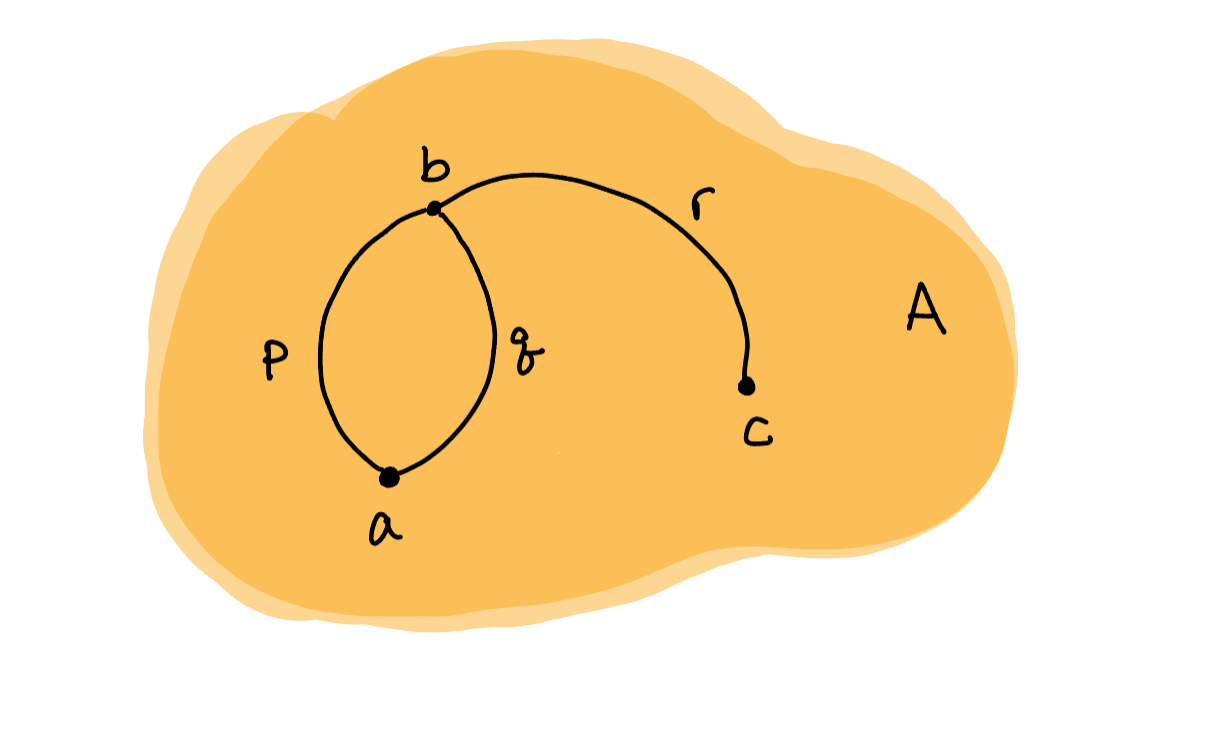
\includegraphics[scale=0.5]{disk.png}
    \caption{A disk-shaped space $A$ and points $a$, $b$, and $c$ and paths $p$, $q$, and $r$.}
    \label{fig:disk}
\end{figure}

\begin{figure}[h]
    \centering
    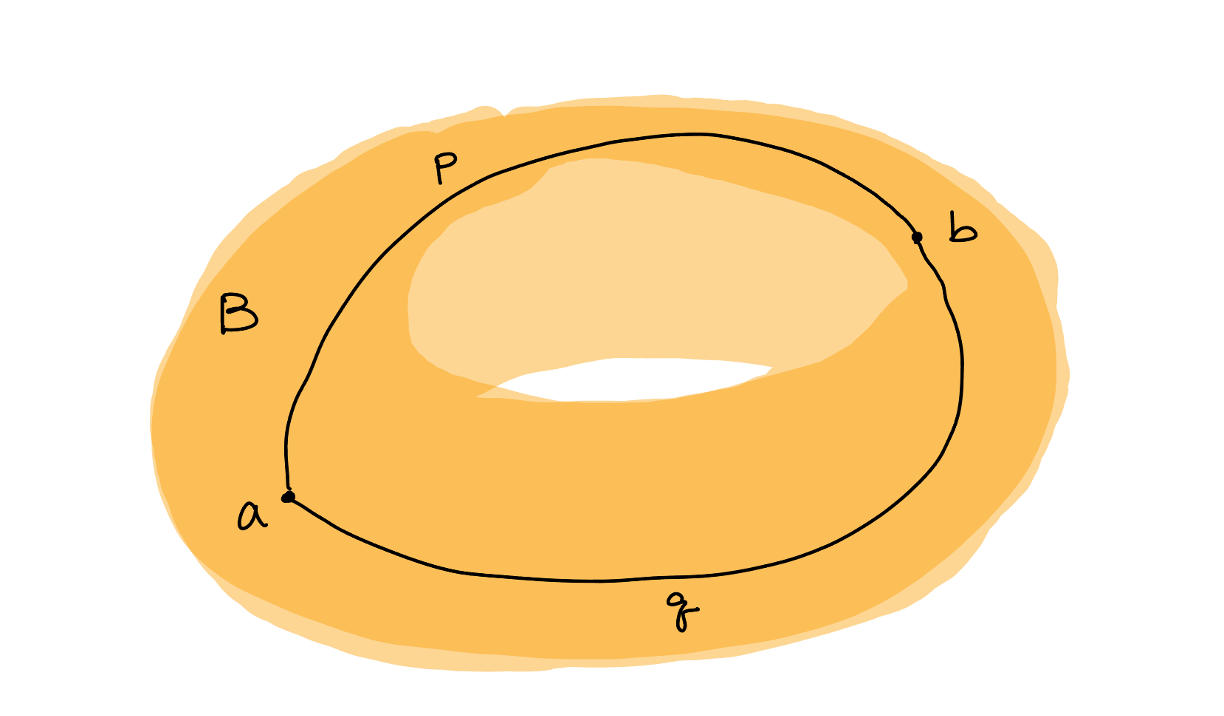
\includegraphics[scale=0.5]{torus.png}
    \caption{A torus-shaped space $B$ and points $a$ and $b$ and paths $p$ and $q$.}
    \label{fig:torus}
\end{figure}

Reflexivity, symmetry, and transitivity of paths suggest groupoidal behaviors of types.

\begin{table}[h]
    \centering
    \begin{tabular}{|c|c|}\hline
        Equality & Homotopy \\\hline
        reflexivity & constant path \\\hline
        symmetry & inverse path \\\hline
        transitivity & path concatenation \\\hline
    \end{tabular}
    \caption{Examples \ref{eg:id-symmetry} and \ref{eg:id-transitivity} reveal the connections between identity types and homotopies.}
    \label{tab:equalities-and-homotopy}
\end{table}

\begin{ex}
    Show that functions $f : A \to B$ respect equalities.
    In other words, construct the following function:
    \[
        \mathsf{ap}_{f} : (a =_{A} b) \to (f(a) =_{B} f(b))
    \]
    The notation $\mathsf{ap}_{f}$ can be read as the \underline{a}ction on \underline{p}aths of $f$ \cite{hottbook}.
\end{ex}

%\begin{figure}[h]
%    \centering
%    \begin{tikzpicture}
\node at (4,0) {$B$};
\node at (5,5) {$\Sigma_{x : B}E(x)$};

\node at (-2,0) {$a$};
\draw[black,fill=black] (-1.5,0) circle (.5ex);

\node at (2.5,0) {$b$};
\draw[black,fill=black] (2,0) circle (.5ex);

\draw (0,5) ellipse (4cm and 1.3cm);
\draw (0,0) ellipse (3cm and 1cm);

\path[draw, snake it] (-1.5,0) -- (2,0);

\node at (0, 0.5) {$p$};

\node at (-2,5) {$f(a)$};
\draw[black,fill=black] (-1.5,5) circle (.5ex);

\node at (2.5,5) {$f(b)$};
\draw[black,fill=black] (2,5) circle (.5ex);

\path[draw, snake it] (-1.5,5) -- (2,5);
\node at (0, 5.5) {$\mathsf{ap}_{f}~p$};

\node at (0.4,2.2) {$\pi_{1}$};
\draw[->] (0,3) -- (0,1.5);
\end{tikzpicture}
%    \caption{Caption}
%    \label{fig:ap}
%\end{figure}

\begin{ex}[Transport]
    Show that for any dependent type $x : B \vdash E(x) \type $, any terms $b, b' : B$, and any path $p : b =_B b'$, there is a function $p_{*} : E(b) \to E(b')$.
\end{ex}
This ensures that every dependent type we can construct respects propositional equality. 
If we think of $E$ as a predicate on $B$, this means that if $E(b)$ is true and $b =_B b'$, then $E(b')$ is true.
This is part of a more sophisticated relationship between type theory and homotopy theory (Quillen model category theory, or QMC theory). 
Transport says that $\pi_{1} : \Sigma_{b : B} E(b) \rightarrow B$ behaves like a fibration in a QMC. For more information, see Appendix $\ref{sec:transport-explanation}$.

\subsection{Functional Extensionality, UIP, and Univalence}

For $\Bool$, we can show that $\False = \False$, $\True = \True$, and that $\False \neq \True$.
For $\N$, we can show that if $S(n) = S(m)$, then $n = m$ for all $n, m : \N$, and that $0 \neq S(n)$ for all $n : \N$.
A more involved example is the $\Sigma$-types, for which we can show that
\[
    \begin{array}{lr}
        (s = t) \simeq \sum_{p : \pi_{1}(s) = \pi_{1}(t)} p_{*}(\pi_{2}(s)) = \pi_{2}(t) & \text{for all } s, t : \sum_{a : A}B(a).
    \end{array}
\]
This roughly says that the identity type $s = t$ is ``equivalent" (a notion that we will introduce later) to the disjoint union of paths in the fibers.

\subsubsection{Functional Extensionality}\label{sec:functional-extensionality}
We consider two set-theoretic functions equal when they are pointwise equal.
This property is called \emph{functional extensionality} (FunExt).
We might want $\Pi$-types to have this property, but this is \textbf{not provable} in MLTT.
However, this is validated by interpretations into logic, sets, and spaces.

\subsubsection{Uniqueness of Identity Proofs}\label{sec:uniqueness-of-identity-proofs}
The \emph{Uniqueness of Identity Proofs} (UIP) states that any two proofs of an identity $p = q$ are equal.
This property is \textbf{not provable} in MLTT.
However, it is validated by interpretations into logic and set, but not in spaces because there may be multiple paths in a space.
See Figure \ref{fig:torus}.

\subsubsection{Univalence}\label{sec:univalence}
From a topologist's perspective, two homeomorphic spaces are equal; from a group theorist's perspective, two isomorphic groups are equal.
Similarly, two equivalent types in a universe $\U$ should be considered equal.
\emph{Univalence} states that
\[
    (T = S) \simeq (T \simeq S)
\]
This is \textbf{not provable} in MLTT, but it is validated by interpretation into \textbf{spaces}.
Univalence is a consequence of the \emph{univalent axiom} (UA), which we will introduce later.

As it turns out, UA and UIP are incompatible, and both UA and UIP imply FunExt.
To avoid inconsistency, we cannot have both UA and UIP. 
We choose UA.
Both choices make sense, but choosing UIP would send us in the direction of set theory, not HoTT.

\begin{figure}[h]
    \centering
    % https://q.uiver.app/#q=WzAsMyxbMCwwLCJVQSJdLFs2LDAsIlVJUCArIEVSIl0sWzMsMywiRnVuRXh0Il0sWzAsMiwiaW1wbGllcyIsMl0sWzEsMiwiaW1wbGllcyJdLFswLDEsImluY29tcGF0aWJsZSIsMCx7InN0eWxlIjp7ImJvZHkiOnsibmFtZSI6InNxdWlnZ2x5In0sImhlYWQiOnsibmFtZSI6Im5vbmUifX19XV0=
\[\begin{tikzcd}
	\mathrm{UA} &&&&&& {\mathrm{UIP \& ER}} \\
	\\
	\\
	&&& \mathrm{FunExt}
	\arrow["\mathrm{Implies}"', from=1-1, to=4-4]
	\arrow["\mathrm{Implies}", from=1-7, to=4-4]
	\arrow["\mathrm{Incompatible}", squiggly, no head, from=1-1, to=1-7]
\end{tikzcd}\]
    \caption{Both UA and UIP with equality reflection (ER) imply functional extensionality.
    However, UA and UIP are incompatible.}
    \label{fig:ua-uip-funext}
\end{figure}

\section{Homotopy Levels}
Types in HoTT come equipped with higher-dimensional structures.
In some types, however, these structures are trivial above a certain dimension.
In this section, we introduce \emph{homotopy levels}, or h-levels for short, and discuss some special cases.

\subsection{h-level 0}\label{sec:h-level-0}
A type $T$ is \emph{contractible} (has h-level 0) if there is a \emph{center of contraction} $t$, and for every inhabitant $s$ of that type there is a path from $s$ to $t$.
\[
    \isContr(T) := \sum_{t : T}\prod_{s : T} (s = t)
\]
\begin{figure}[h]
    \centering
    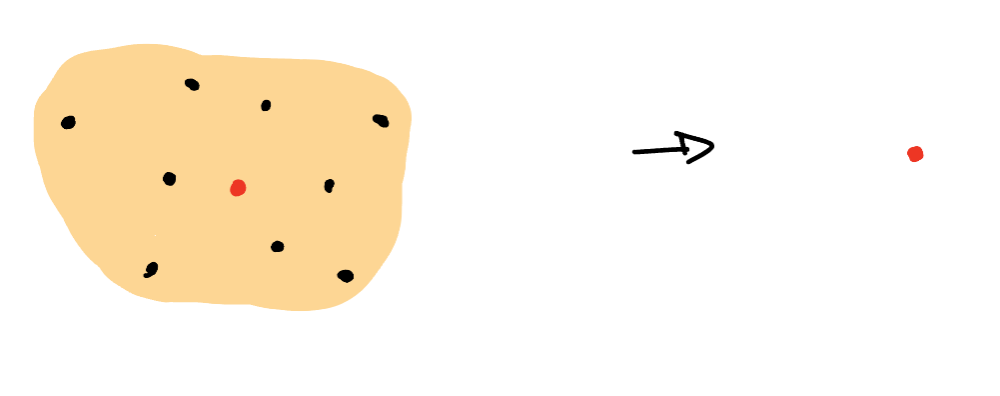
\includegraphics[scale=0.5]{hlvl0.png}
    \caption{A type $T$ with h-level 0 has a center of contraction $t$ and every inhabitant has a path to $t$.}
    \label{fig:h-level-0}
\end{figure}

For example, the unit type $\Unit$ is contractible.
Choose $\mathsf{tt}$ to be the center of contraction.
The result follows by the elimination rule for $\Unit$.

\begin{ex}
Show that if $T$ is contractible and inhabited, then $T \simeq \mathbbm{1}$.
\end{ex}

%\begin{figure}[h]
%    \centering
%    \begin{tikzpicture}
    \draw (0,0) circle (3cm);
    \node (t) at (0,0) {};
    \draw[black, fill=black] (0, 0) circle (.5ex);

    \node (1) at (2,2) {};
    \node (2) at (-1.3,1) {};
    \node (3) at (-2.3,-0.3) {};
    \node (4) at (1.7,-2);

    \draw[->] (1) -- (t);
    \draw[->] (2) -- (t);
    \draw[->] (3) -- (t);
    \draw[->] (4) -- (t);
\end{tikzpicture}
%    \caption{Caption}
%    \label{fig:h-level0}
%\end{figure}

\subsection{h-level 1}\label{sec:h-level-1}
A type $T$ is a \emph{proposition} (has h-level 1) if for any $s, t : T$ the identity type $s = t$ is contractible.
\[
    \isProp(T) := \prod_{s,t : T}\isContr(s = t)
\]
Note that a proposition does not need to be inhabited.
For example, the empty type $\varnothing$ is a proposition.
See Exercise \ref{ex:empty-unit-prop}.
\begin{figure}[h]
    \centering
    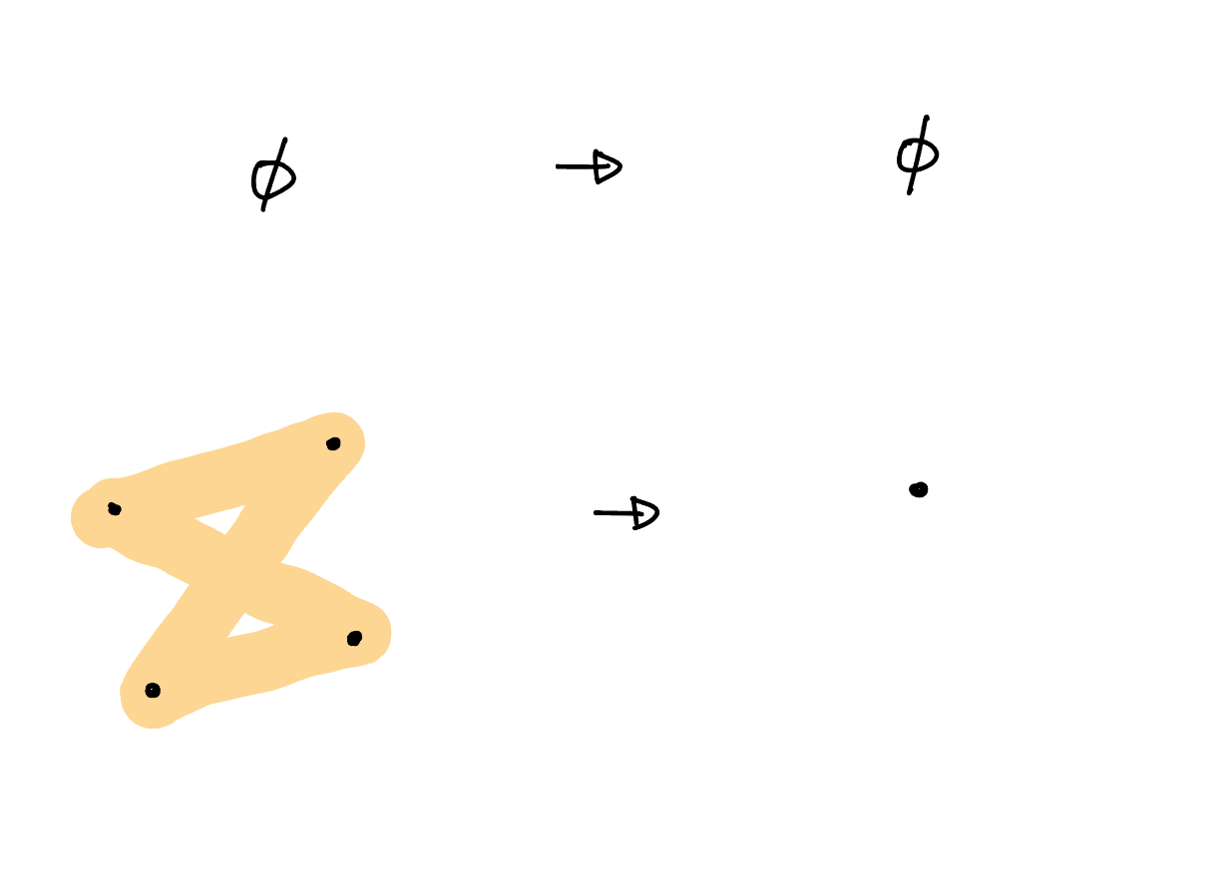
\includegraphics[scale=0.5]{hlvl1.png}
    \caption{If a type $T$ has h-level 1, then the identity type $s = t$ between any two inhabitants $s$ and $t$ is contractible.
    This means that any two proofs of a proposition are equal.}
    \label{fig:h-level-1}
\end{figure}

\begin{ex}\label{ex:empty-unit-prop}
Show that $\emptyset$, $\mathbbm{1}$ are propositions.
\end{ex}

\begin{ex}
Show that any contractible type is a proposition.
\end{ex}

\begin{ex}
Show that if a proposition is inhabited, then it is contractible. (This says that a proposition is informally equivalent to $\varnothing$ or $\mathbbm{1}$, i.e., truth values) %I don't think this is actually what this exercise shows but I'm not sure what the correct interpretation of this comment in the notes is
\end{ex}

\subsection{h-level 2}\label{sec:h-level-2}
A type $T$ is a \emph{set} (has h-level 2) if for any $s, t : T$ the identity type $s = t$ is a proposition.
\[
    \isSet(T) := \prod_{s,t : T}\isProp(s = t)
\]
The type $T$ looks like a discrete collection of points.
For example, the types $\N$ and $\Bool$ are sets.
\begin{figure}[h]
    \centering
    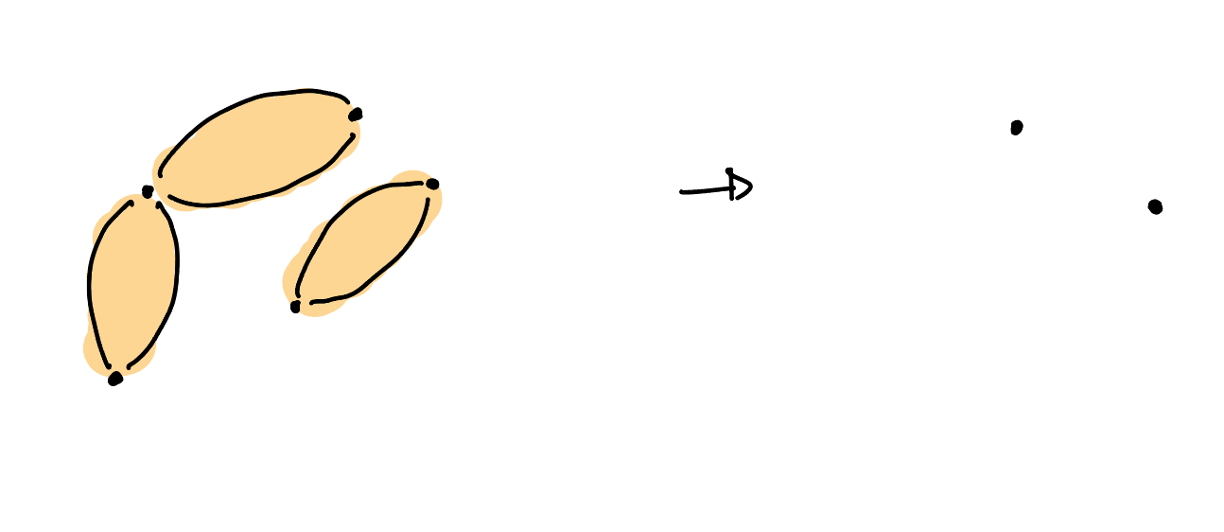
\includegraphics[scale=0.5]{hlvl2.png}
    \caption{If a type $T$ has h-level 2, then the identity type $s = t$ between any two inhabitants $s$ and $t$ is a proposition.
    Thus, $T$ looks like a set.}
    \label{fig:h-level-2}
\end{figure}

\subsection{h-level 3}\label{sec:h-level-3}
A type $T$ is a \emph{groupoid} (has h-level 3) if for any $s, t : T$ the identity type $s = t$ is a set.
\[
    \isGroupoid(T) := \prod_{s, t : T}\isSet(s = t)
\]
\begin{figure}[h]
    \centering
    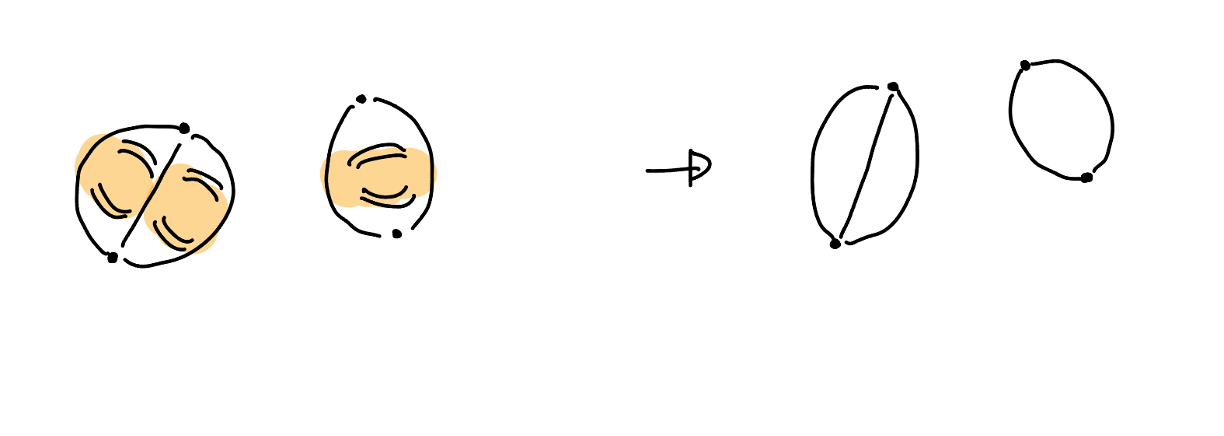
\includegraphics[scale=0.5]{hlvl3.png}
    \caption{If a type $T$ has h-level 3, then the identity type $s = t$ between any two inhabitants $s$ and $t$ is a set.
    Thus, $T$ looks like a groupoid.}
    \label{fig:h-level-3}
\end{figure}

In general, $\isofhlevel{n}{T}$ is defined recursively as follows:
\begin{align*}
    \isofhlevel{0}{T} &:= \isContr(T)\\
    \isofhlevel{S(n)}{T} &:= \prod_{s,t : T}\isofhlevel{n}{(s = t)}
\end{align*}

\begin{ex}
Show that if a type $T$ has h-level $n$, then it has h-level $n + 1$.
\end{ex}

\section{Equivalences}
Given a function $f : A \to B$, we can define $\isEquiv(f)$ by
\[
    \sum_{g : B \to A} (g \circ f = 1_{A}) \times (f \circ g = 1_{B})
\]
Sadly, this type is not a proposition.
Thus, it has nontrivial high-dimensional structures that we don't want.
To remedy this, recall that a set-theoretic function $f : A \to B$ is a bijection if for all $b \in B$, the fiber over $b$ is a singleton set.
This suggests an alternative definition for $\isEquiv(f)$.
\begin{defn}
\begin{align*}
    \isEquiv(f) &:= \prod_{b : B} \isContr\left(\sum_{a : A} f(a)=b\right)
\end{align*}
\end{defn}
This states that for every $b : B$, the fiber over $b$ is contractible, i.e., there exists a unique element in the preimage of $f$.
One can prove that $\isEquiv(f)$ is a proposition.

\begin{defn}[Equivalence]
    Given any two types $A, B : \U$, we write $A \simeq B$ to denote the type $\displaystyle\sum_{f : A \to B} \isEquiv(f)$.
\end{defn}
For any two types $A, B : \U$, we can construct a function $\idToEquiv : (A = B) \to (A \simeq B)$ by path induction.
\begin{defn}[Univalence Axiom]
    The \emph{univalence axiom} asserts that 
    \[\ua : \isEquiv(\idToEquiv)\]
\end{defn}
An immediate consequence of this axiom is that $(A = B) \simeq (A \simeq B)$.

\subsection{Univalence for Logic and Sets}\label{sec:univalence-for-logic-and-sets}
\begin{defn}
    We define the type of propositions as the following sigma type:
    \[\Prop := \sum_{P : \U} \isProp(P)\]
\end{defn}
The univalence axiom implies that the type $\Prop$ is univalent.
That is, for any $P, Q : \Prop$,
\[
    (P = Q) \simeq (P \leftrightarrow Q)
\]
As a corollary, the type $\Prop$ is a set rather than a proposition because there are propositions that are not interprovable, but all the interprovable ones can be identified.
We define the type of sets in the same fashion.
\begin{defn}
\[
    \Set := \sum_{S : \U} \isSet(S)
\]
\end{defn}
Similarly, the univalence axiom implies that $\Set$ is univalent.
\[
    (S = T) \simeq (S \cong T)
\]
As a consequence, $\Set$ is a groupoid because, for example, the set containing two elements is isomorphic to itself in two different ways.

With $\Set$ in hand, we can define the type of groups.
Recall that a group consists of a carrier set $G$, a neutral element $e$, a multiplication operator $\cdot$, and an inverse operator $-^{-1}$ such that
\begin{enumerate}
    \item $e \cdot g = g$ for all $g \in G$,
    \item $g \cdot e = g$ for all $g \in G$,
    \item $(g \cdot h) \cdot k = g \cdot (h \cdot k)$ for all $g, h, k \in G$,
    \item $g^{-1} \cdot g = e$ for all $g \in G$, and
    \item $g \cdot g^{-1} = e$ for all $g \in G$.
\end{enumerate}
\begin{defn}
    \begin{align*}
        \Grp := \sum_{G : \Set}&\sum_{e : G}\sum_{\cdot : G \to G \to G}\sum_{-^{-1} : G \to G}\left(\prod_{g : G} e \cdot g = g\right) \times\\
        &\left(\prod_{g : G} g \cdot e = g\right) \times \left(\prod_{g,h,k : G}(g \cdot h) \cdot k = g \cdot (h \cdot k)\right) \times\\
        &\left(\prod_{g : G}g^{-1} \cdot g = e\right) \times \left(\prod_{g : G}g \cdot g^{-1} = e\right)
    \end{align*}
\end{defn}
The role of the inhabitants of the group axioms is to serve as a \emph{witness} that the neutral element, the multiplication, and the inverse of a group interact properly.
We don't want the group axioms to carry additional structures.
Thus, the carrier $G$ needs to be a set to ensure that the group axioms are propositions.

%This encodes the existence of an identity ($e$), a partial binary operator ($m$), and an inverse operator $i$ satisfying the groupoid axioms ($e$ acts as an identity, $m$ is associative, and %inverses act as inverses). %is m partial? this seems like it's actually a group not a groupoid?

Again, the univalence axiom implies that for any two groups, $G$ and $H$,
\[(G = H)\simeq (G \cong H).\]
Similarly, we can define the type of groupoids by
\[\Grpd:= \sum_{T:\U} \isGroupoid(T)\]
And the type $\Grpd$ is univalent.
In fact, any algebraic structure on a set has a univalence result \cite{coq:isomorphism-is-equality}.

%\textsc{Definition.} An algebraic structure is %needs definition from github once paige adds it there

The moral of the story is that univalence allows us to do mathematics up to some appropriate notion of ``sameness".
For example, the appropriate notion of sameness for groups is group isomorphisms.
The \textbf{Structure Identity Principle}, or \textbf{SIP} (Aczel, Coqand), is the idea that an isomorphism (or our notions of equivalence) should respect the structure of a given type.
The \textbf{Identity of Indiscernables} (Leibniz) states that any two objects that have all their properties in common cannot be distinct.
Univalence allows us to treat equivalent types as exactly equal, incorporating these principles into our theory.

\section{Higher Inductive Types}
An ordinary inductive type, such as $\Bool$, is freely generated by its canonical terms $\True$ and $\False$.
Since we now consider types as having terms, equalities, equalities between equalities, etc, we can consider \emph{higher inductive types} whose constructors can generate terms, equalities, equalities between equalities, etc.
For example, we can define the type $D^{1}$ to be the higher inductive type generated by two points $\bullet$ and $\star$, and a path between them $p : \bullet = \star$.
The topological intuition here is that we connect the points $\bullet$ and $\star$ by adding the path $p$. 
($S^0$ is the $0$-dimensional sphere, and $D^1$ is the the $1$-dimensional disc.)

\begin{mathpar}
    \inferrule*[Right=Form]
    { }
    { \vdash D^{1} \type }\and

    \inferrule*[Right=Intros]
    { }
    { \vdash \bullet : D^{1} \and \vdash \star : D^{1} \and \vdash p : \bullet = \star }\and

    \inferrule*[Right=Elim]
    { x : D^{1} \vdash E(x) \type\\
      \vdash t : E(\bullet)\\
      \vdash f : E(\star)\\
      \vdash \pi : p_{*}t = f
    }
    { x : D^{1} \vdash \Ind_{D^{1},t,f,\pi}(x) : E(x) }\and

    \inferrule*[Right=Comp]
    { x : D^{1} \vdash E(x) \type\\
      \vdash t : E(\bullet)\\
      \vdash f : E(\star)\\
      \vdash \pi : p_{*}t = f
    }
    { \vdash \Ind_{D^{1},t,f,\pi}(\bullet) \defeq t : E(\bullet) \and
      \vdash \Ind_{D^{1},t,f,\pi}(\star) \defeq f : E(\star) \\\\
      \vdash \Ind_{D^{1},t,f,\pi}(p) = \pi : p_{*}t = f }
\end{mathpar}

We explore a few more higher inductive types.

\subsection{Propositional Truncation}\label{sec:propositional-truncation}
Given two propositions $P$ and $Q$, we can prove that the types $P \times Q$, $P \to Q$, and $\lnot P$ are propositions.
Thus, we can define conjunctions, implications, and negations in the most obvious way.
However, $P + Q$ is not necessarily a proposition since if we have $p : P$ and $q : Q$, then we have $\inl(p) : P + Q$ and $\inr(q) : P + Q$.
We can turn this into a proposition by identifying $\inl(p)$ and $\inr(q)$.
\begin{defn}
    In general, given a type $T$, the \emph{propositional truncation} $\| T \|_1$ of $T$ is the higher inductive type generated by an injection $\vert\cdot\vert_{1} : T \to \| T \|_{1}$ and a path identifying any pair of inhabitants:
    \[
        p : \prod_{x,y : T}\vert x \vert_{1} = \vert y \vert_{1}
    \]
\end{defn}
With this, we can define $P \lor Q := \| P + Q \|_{1}$.

\begin{ex}
    Show that for all $T$, $\isProp(\| T \|_1)$.
\end{ex}

\subsection{Set Truncation}\label{sec:set-truncation}
We can define the type of circles $S^{1}$ to be the higher inductive type generated by a base point $b : S^{1}$ and a loop $\ell : b = b$.
A classical result in algebraic topology is that the fundamental group of the circle is isomorphic to $\Z$.
Indeed, we have that
\[
    \pi_{1}(S^{1}) \simeq \Z
\]
We define $\pi_{1}(T, t) := (S^{1}, b) \to (T, t)$ to be the ``set" of base-perserving functions.
However, there no reason for this type to be a set.
Set truncation allows us to remedy this.
\begin{defn}
    Given a type $T$, the \emph{set truncation} $\| T \|_2$ of $T$ is the higher inductive type generated by an injection $\vert \cdot \vert_2 : T \to \| T \|_2$, and a 2-path identifying any two 1-paths:
    \[p : \prod_{x,y : T}\prod_{p,q : x = y} \vert p \vert_2 = \vert q \vert_2\]
\end{defn}
Now, we can define $\| \pi_{1}(T, t) := (S^{1}, b) \to (T, t) \|_{2}$.
\begin{ex}
    Show that for all $T$, $\isSet(\| T \|_2)$.
\end{ex}

\subsection{Quotient Types}\label{sec:quotient-types}
\begin{defn}
    Given an equivalence relation $\sim$ on a set $S$, we can take the \emph{quotient} $S/\sim$ to be the higher inductive type given by:
    \begin{itemize}
        \item an injection $\iota : S \to S/\sim$;
        \item a dependent function $j : \prod_{x, y : S} x \sim y \to \iota(x) = \iota(y)$;
        \item constructors for $\| \cdot \|_2$.
    \end{itemize}
\end{defn}

\section{Category Theory}

Traditionally, a category $\cat{C}$ consists of
\begin{enumerate}
    \item a set $\ob{C}$ of objects,
    \item a set $\cHom{X}{Y}$ of morphisms for all $X, Y \in \ob{C}$,
    \item an identity morphism $\cId_{X} \in \cHom{X}{X}$ for all $X \in \ob{C}$,
    \item a composition function $\circ : \cHom{Y}{Z} \to \cHom{X}{Y} \to \cHom{X}{Z}$ for all $X, Y, Z \in \ob{C}$.
\end{enumerate}
These data are subject to the identity and associativity laws.

We could talk about categories in the set level (like most classical mathematics).
However, the structural identity principle for structures on sets tells us that 
\[(\cat{C} =_{\Cat} \cat{D}) \simeq (\cat{C} \cong \cat{D}).\]
But isomorphism is not the right kind of sameness for categories; they are too strong.
Instead of squashing everything down to the level of sets, HoTT affords higher dimensional structures.

\subsection{Univalent Categories}\label{sec:univalent-categories}
Observe that every category has a ``core groupoid" contained within it: the objects and all isomorphisms.
With a groupoid of objects in hand, we can then glue additional morphisms to this groupoid, forming a category.
\begin{defn}
    A \emph{univalent category} $\cat{C}$ consists of:
\begin{itemize}
    \item a groupoid of objects $\ob{C} : \Grpd$;
    \item a set $\cHom{X}{Y}$ for every pair $X,Y : \ob{C}$, i.e., $$X,Y : \ob{C} \vdash \cHom{X}{Y} : \Set;$$
    \item a term $\cId_{X} : \cHom{X}{X}$ for every $X : \ob{C}$, i.e., $$X:\ob{C} \vdash \cId_{X} : \cHom{X}{X};$$
    \item a function $\circ: \cHom{Y}{Z} \to \cHom{X}{Y} \to \cHom{X}{Z}$ for every $X,Y,Z : \ob{C}$, i.e., $$X,Y,Z: \ob{C} \vdash \circ : \cHom{X}{Y} \to \cHom{Y}{Z}\to \cHom{X}{Z}$$
\end{itemize}
These data are subject to the usual axioms of categories and that the function
\[
    \idToIso: (X=Y) \to \Iso(X,Y)
\]
is an equivalence, where 
$$\Iso(X,Y) := \sum_{f:\cHom{X}{Y}} \sum_{g:\cHom{Y}{X}} (g\circ f = \cId_{X}) \times (f \circ g = \cId_{Y}).$$
Thus, the right notion of sameness for objects is isomorphism.
This additional requirement is often called (internal) univalence.
\end{defn}
The type of categories $\Cat$ can then be defined as an iterated sigma type.
As a consequence of the univalence axiom,
\[
    (\cat{C} =_{\Cat} \cat{D}) \simeq (\cat{C} \simeq \cat{D}).
\]
Thus, the terms of $\Cat$ are categories and the equalities are equivalence of categories.
\begin{cor}
    $\Cat$ is a $2$-groupoid (h-level $4$).
\end{cor}
This is a great achievement for the univalent foundations.
Category theorists call definitions that are not invariant under equivalence of categories \emph{evil}.
This definition helps us avoid ``evilness" when we talk about categories.

%We now define functors and natural transformations. 
%\begin{defn}
%    A \emph{functor} $F: \cat{C}\to\cat{D}$ consists of:
%\begin{itemize}
%    \item a function $\ob{F}: \ob{C}\to \ob{D}$;
%    \item functions $\hom_{\mathbf C}(X,Y)\to \hom_{\mathbf D}(FX,FY)$ for all $X,Y\in \mathbf C$
%\end{itemize}
%such that the compositions and identities are preserved.
%\end{defn}

%The type of functors $[\mathcal C, \mathcal D]$ is not a set.
%\begin{enumerate}
%    \item terms $\rightsquigarrow$ functions;
%    \item equalities $\rightsquigarrow$ natural transformations.
%\end{enumerate}

%\begin{defn}
%    A \emph{natural transformation} $\eta: F \implies G: \mathbf{C}\to\mathbf{D}$ consists of $\eta_X:\hom(FX,GX)$ for all $X:\ob{C}$ such that the following square commutes for all %$X,Y:\ob{C}$ and all $f:\hom(X,Y)$:

%\begin{center}
%\begin{tikzcd}
%FX \arrow[r, "Ff"] \arrow[d, "\eta_X"]
%& FY \arrow[d, "\eta_Y"] \\
%GX \arrow[r, "Gf"]
%& || GY
%\end{tikzcd}
%\end{center}
%\end{defn}

%The type of natural transformations $F\implies G$ is a set.

%We can also form a \emph{bicategory} of categories. We have univalence for bicategories, as well as for any higher (but finite) algebraic structure.

\subsection{Rezk Completion}\label{sec:rezk-completion}
A \emph{precategory} is a univalent category except that the type of objects $\ob{C}$ is not necessarily a groupoid, and that internal univalence is not assumed.
There is a canonical way of turning a precategory into a univalent one.
\begin{defn}
    The \emph{Rezk completion} of a precategory $\cat{C}$ takes $\ob{\Rezk(C)}$ to be the higher inductive type given by:
    \begin{itemize}
        \item an injection $\iota : \ob{C} \to \ob{\Rezk(C)}$;
        \item a dependent function $j : \prod_{X, Y : \ob{C}} \Iso(X,Y) \to \iota(X) = \iota(Y)$;
        \item constructors for $\| \cdot \|_3$
    \end{itemize}
\end{defn}

\bibliographystyle{alpha}
\bibliography{all}

\appendix

\section{Transport and Fibrations}
\label{sec:transport-explanation}

As mentioned earlier, the ability to transport along an equality corresponds to the projection map $\pi_1 : \Sigma_{b : B} E(b)$ behaving like a fibration in a QMC. We will now discuss one way to see this, taking the liberty to interpret equalities as a map from the interval type into the target type, as is possible in a QMC (as well as in cubical formulations of HoTT).

\begin{figure}[h]
    \centering
    % https://q.uiver.app/#q=WzAsNCxbMCwwLCIqIl0sWzIsMCwiXFxTaWdtYV97YiA6IEJ9IEUoYikiXSxbMCwyLCJJIl0sWzIsMiwiQiJdLFsyLDMsInAiLDJdLFswLDEsIlxcdGV4dHtjb25zdH1feyhiLCBlKX0iXSxbMCwyLCJcXHRleHR7Y29uc3R9X3swfSIsMl0sWzEsMywiXFxwaV8xIl0sWzIsMSwiaCIsMix7InN0eWxlIjp7ImJvZHkiOnsibmFtZSI6ImRhc2hlZCJ9fX1dXQ==
\[\begin{tikzcd}
	{*} && {\Sigma_{b : B} E(b)} \\
	\\
	I && B
	\arrow["p"', from=3-1, to=3-3]
	\arrow["{\text{const}_{(b, e)}}", from=1-1, to=1-3]
	\arrow["{\text{const}_{0}}"', from=1-1, to=3-1]
	\arrow["{\pi_1}", from=1-3, to=3-3]
	\arrow["h"', dashed, from=3-1, to=1-3]
\end{tikzcd}\]
    \caption{Given that the outer diagram commutes, we have that if $\pi_1$ is a fibration, there exists a homotopy lifting map $h$ making everything commute.}
    \label{fig:transport-as-fibration}
\end{figure}

Consider Figure \ref{fig:transport-as-fibration}. If the outer diagram commutes, we have the data $b : B$, $e : E(b)$, and a path $p : b = b'$ for some (unstated) $b' : B$.

This follows because, when interpreting $p$ as a map from $I$ to $B$, evaluating $p$ at $0 : I$ must result in $b$ by commutativity.

Then, if $\pi_1$ is a fibration, we get that there exists a homotopy lift $h : (b, e) = (b', e')$ for some (unstated) $e' : E(b')$ that makes the diagram commute.

This is because, when interpreting $h$ as a map from $I$ to $\Sigma_{b : B} E(b)$, evaluating $p$ at $0 : I$ must result in $(b, e)$ by commutativity.

Furthermore, evaluating $h$ at $1 : I$ and then applying $\pi_1$ must result in the same value as evaluating $p$ at $1 : I$, also by commutativity.

Thus, given such an $h$, we can define $tr_p (e)$ to equal $\pi_2 (h (1)) : E(b')$. Thus, if $\pi_1$ is always a fibration, given a term $p : b = b'$, we can define $tr_p : E(b) \to E(b')$.

In the reverse direction, given a term $tr_p : E(b) \to E(b')$ along with the property that $tr_{r_b} \defeq \text{id}_{E(b)}$ (which holds when defining transport using path induction), given that the outer diagram in Figure \ref{fig:transport-as-fibration} commutes, we can define $h : (b, e) = (b', tr_p (e))$.

To do this, we can use the elimination rule for identity types to reduce this problem to the case where $b' \defeq b$ and $p \defeq r_b$. As such, we now want to define $h : (b, e) = (b', tr_{r_b} (e))$.

But as $(b', tr_{r_b} (e))$ definitionally reduces to $(b, \text{id}_{E(b)} (e))$ and then again to $(b, e)$, we get that $h : (b, e) = (b, e)$.

As such, we can just let $h$ be $r_{(b, e)}$ to finish the proof.

Thus, we have that if $\pi_1$ is a fibration, we can construct transport along a path $p : b = b'$ as $tr_b : E(b) \to E(b')$, and if we have transport we can show that $\pi_1$ is a fibration.

As a bonus exercise, prove that this map taking in $tr_p$ and output $h$ is an equivalence!

\section{Digression: Pi-Types}
$\prod$-types are dependent function types. 
Note that they are \textbf{not} an inductive type, but we include a sketch of the rules for them here.

\begin{mathpar}
    \inferrule*[Right=Form]
    {x : B \vdash E(x) \type}
    {\vdash \prod_{x : B} E(x) \type}\and

    \inferrule*[Right=Intros]
    {x : B \vdash e : E(x)}
    {\vdash \lambda x : B.~e : \prod_{x : B}E(x)}\and

    \inferrule*[Right=Elim]
    { \vdash f : \prod_{x : B} E(x)\\
      \vdash b : B
    }
    { \vdash f~b : E(b) }\and

    \inferrule*[Right=Comp]
    { x : B \vdash e : E(x)\\
      \vdash b : B }
    { \vdash (\lambda x : B.~e)~b \defeq e[b/x] : E(b) }\and

    \inferrule*[Right=Uniq]
    { \vdash f : \prod_{x : B} E(x) }
    { \vdash f \defeq (\lambda x : B.~f~x) : \prod_{x : B} E(x) }
\end{mathpar}

\section{Links and FAQ}

\begin{enumerate}
    \item \textbf{How does univalence imply functional extensionality?} Here is a blog post detailing that: \href{https://homotopytypetheory.org/2014/02/17/another-proof-that-univalence-implies-function-extensionality/}{Another proof that univalence implies functional extensionality by Dan Licata}.

    Perhaps the biggest takeaway from this article is that this proof that univalence implies functional extensionality is very closely related to the proof in cubical type theory of functional extensionality, which doesn't use univalence! There is something bigger at play here, demonstrating that univalence in some way makes things in MLTT "work better" than it used to.

    Other than that, I highly recommend checking out the article linked above, as it is by far the clearest explanation of this proof that I've seen.
    \item \textbf{Are h-levels different from universe levels?} Yes! In a type hierarchy such as the one used by Coq, each $\texttt{Type}_i$ has h-level $\infty$.
    \item \textbf{How does the inductive definition of identity types allow for non-canonical terms?} The crucial difference for identity types is that we are inductively defining a \textit{family} of types in \ref{sec:identity}. The types build by these definitions are indexed by the terms being equated, allowing us to have non-canonical terms.
\end{enumerate}

\end{document}
